\documentclass[11pt]{article}

    \usepackage[breakable]{tcolorbox}
    \usepackage{parskip} % Stop auto-indenting (to mimic markdown behaviour)
    
    \usepackage{iftex}
    \ifPDFTeX
    	\usepackage[T1]{fontenc}
    	\usepackage{mathpazo}
    \else
    	\usepackage{fontspec}
    \fi

    % Basic figure setup, for now with no caption control since it's done
    % automatically by Pandoc (which extracts ![](path) syntax from Markdown).
    \usepackage{graphicx}
    % Maintain compatibility with old templates. Remove in nbconvert 6.0
    \let\Oldincludegraphics\includegraphics
    % Ensure that by default, figures have no caption (until we provide a
    % proper Figure object with a Caption API and a way to capture that
    % in the conversion process - todo).
    \usepackage{caption}
    \DeclareCaptionFormat{nocaption}{}
    \captionsetup{format=nocaption,aboveskip=0pt,belowskip=0pt}

    \usepackage[Export]{adjustbox} % Used to constrain images to a maximum size
    \adjustboxset{max size={0.9\linewidth}{0.9\paperheight}}
    \usepackage{float}
    \floatplacement{figure}{H} % forces figures to be placed at the correct location
    \usepackage{xcolor} % Allow colors to be defined
    \usepackage{enumerate} % Needed for markdown enumerations to work
    \usepackage{geometry} % Used to adjust the document margins
    \usepackage{amsmath} % Equations
    \usepackage{amssymb} % Equations
    \usepackage{textcomp} % defines textquotesingle
    % Hack from http://tex.stackexchange.com/a/47451/13684:
    \AtBeginDocument{%
        \def\PYZsq{\textquotesingle}% Upright quotes in Pygmentized code
    }
    \usepackage{upquote} % Upright quotes for verbatim code
    \usepackage{eurosym} % defines \euro
    \usepackage[mathletters]{ucs} % Extended unicode (utf-8) support
    \usepackage{fancyvrb} % verbatim replacement that allows latex

    % The hyperref package gives us a pdf with properly built
    % internal navigation ('pdf bookmarks' for the table of contents,
    % internal cross-reference links, web links for URLs, etc.)
    \usepackage{hyperref}
    % The default LaTeX title has an obnoxious amount of whitespace. By default,
    % titling removes some of it. It also provides customization options.
    \usepackage{titling}
    \usepackage{longtable} % longtable support required by pandoc >1.10
    \usepackage{booktabs}  % table support for pandoc > 1.12.2
    \usepackage[inline]{enumitem} % IRkernel/repr support (it uses the enumerate* environment)
    \usepackage[normalem]{ulem} % ulem is needed to support strikethroughs (\sout)
                                % normalem makes italics be italics, not underlines
    \usepackage{mathrsfs}
    

    
    % Colors for the hyperref package
    \definecolor{urlcolor}{rgb}{0,.145,.698}
    \definecolor{linkcolor}{rgb}{.71,0.21,0.01}
    \definecolor{citecolor}{rgb}{.12,.54,.11}

    % ANSI colors
    \definecolor{ansi-black}{HTML}{3E424D}
    \definecolor{ansi-black-intense}{HTML}{282C36}
    \definecolor{ansi-red}{HTML}{E75C58}
    \definecolor{ansi-red-intense}{HTML}{B22B31}
    \definecolor{ansi-green}{HTML}{00A250}
    \definecolor{ansi-green-intense}{HTML}{007427}
    \definecolor{ansi-yellow}{HTML}{DDB62B}
    \definecolor{ansi-yellow-intense}{HTML}{B27D12}
    \definecolor{ansi-blue}{HTML}{208FFB}
    \definecolor{ansi-blue-intense}{HTML}{0065CA}
    \definecolor{ansi-magenta}{HTML}{D160C4}
    \definecolor{ansi-magenta-intense}{HTML}{A03196}
    \definecolor{ansi-cyan}{HTML}{60C6C8}
    \definecolor{ansi-cyan-intense}{HTML}{258F8F}
    \definecolor{ansi-white}{HTML}{C5C1B4}
    \definecolor{ansi-white-intense}{HTML}{A1A6B2}
    \definecolor{ansi-default-inverse-fg}{HTML}{FFFFFF}
    \definecolor{ansi-default-inverse-bg}{HTML}{000000}

    % commands and environments needed by pandoc snippets
    % extracted from the output of `pandoc -s`
    \providecommand{\tightlist}{%
      \setlength{\itemsep}{0pt}\setlength{\parskip}{0pt}}
    \DefineVerbatimEnvironment{Highlighting}{Verbatim}{commandchars=\\\{\}}
    % Add ',fontsize=\small' for more characters per line
    \newenvironment{Shaded}{}{}
    \newcommand{\KeywordTok}[1]{\textcolor[rgb]{0.00,0.44,0.13}{\textbf{{#1}}}}
    \newcommand{\DataTypeTok}[1]{\textcolor[rgb]{0.56,0.13,0.00}{{#1}}}
    \newcommand{\DecValTok}[1]{\textcolor[rgb]{0.25,0.63,0.44}{{#1}}}
    \newcommand{\BaseNTok}[1]{\textcolor[rgb]{0.25,0.63,0.44}{{#1}}}
    \newcommand{\FloatTok}[1]{\textcolor[rgb]{0.25,0.63,0.44}{{#1}}}
    \newcommand{\CharTok}[1]{\textcolor[rgb]{0.25,0.44,0.63}{{#1}}}
    \newcommand{\StringTok}[1]{\textcolor[rgb]{0.25,0.44,0.63}{{#1}}}
    \newcommand{\CommentTok}[1]{\textcolor[rgb]{0.38,0.63,0.69}{\textit{{#1}}}}
    \newcommand{\OtherTok}[1]{\textcolor[rgb]{0.00,0.44,0.13}{{#1}}}
    \newcommand{\AlertTok}[1]{\textcolor[rgb]{1.00,0.00,0.00}{\textbf{{#1}}}}
    \newcommand{\FunctionTok}[1]{\textcolor[rgb]{0.02,0.16,0.49}{{#1}}}
    \newcommand{\RegionMarkerTok}[1]{{#1}}
    \newcommand{\ErrorTok}[1]{\textcolor[rgb]{1.00,0.00,0.00}{\textbf{{#1}}}}
    \newcommand{\NormalTok}[1]{{#1}}
    
    % Additional commands for more recent versions of Pandoc
    \newcommand{\ConstantTok}[1]{\textcolor[rgb]{0.53,0.00,0.00}{{#1}}}
    \newcommand{\SpecialCharTok}[1]{\textcolor[rgb]{0.25,0.44,0.63}{{#1}}}
    \newcommand{\VerbatimStringTok}[1]{\textcolor[rgb]{0.25,0.44,0.63}{{#1}}}
    \newcommand{\SpecialStringTok}[1]{\textcolor[rgb]{0.73,0.40,0.53}{{#1}}}
    \newcommand{\ImportTok}[1]{{#1}}
    \newcommand{\DocumentationTok}[1]{\textcolor[rgb]{0.73,0.13,0.13}{\textit{{#1}}}}
    \newcommand{\AnnotationTok}[1]{\textcolor[rgb]{0.38,0.63,0.69}{\textbf{\textit{{#1}}}}}
    \newcommand{\CommentVarTok}[1]{\textcolor[rgb]{0.38,0.63,0.69}{\textbf{\textit{{#1}}}}}
    \newcommand{\VariableTok}[1]{\textcolor[rgb]{0.10,0.09,0.49}{{#1}}}
    \newcommand{\ControlFlowTok}[1]{\textcolor[rgb]{0.00,0.44,0.13}{\textbf{{#1}}}}
    \newcommand{\OperatorTok}[1]{\textcolor[rgb]{0.40,0.40,0.40}{{#1}}}
    \newcommand{\BuiltInTok}[1]{{#1}}
    \newcommand{\ExtensionTok}[1]{{#1}}
    \newcommand{\PreprocessorTok}[1]{\textcolor[rgb]{0.74,0.48,0.00}{{#1}}}
    \newcommand{\AttributeTok}[1]{\textcolor[rgb]{0.49,0.56,0.16}{{#1}}}
    \newcommand{\InformationTok}[1]{\textcolor[rgb]{0.38,0.63,0.69}{\textbf{\textit{{#1}}}}}
    \newcommand{\WarningTok}[1]{\textcolor[rgb]{0.38,0.63,0.69}{\textbf{\textit{{#1}}}}}
    
    
    % Define a nice break command that doesn't care if a line doesn't already
    % exist.
    \def\br{\hspace*{\fill} \\* }
    % Math Jax compatibility definitions
    \def\gt{>}
    \def\lt{<}
    \let\Oldtex\TeX
    \let\Oldlatex\LaTeX
    \renewcommand{\TeX}{\textrm{\Oldtex}}
    \renewcommand{\LaTeX}{\textrm{\Oldlatex}}
    % Document parameters
    % Document title
    \title{Airplane allocation - A stochastic problem}
    \author{THOMINET Benjamin - REVERSAT Valentin}
    \date{Autumn semester - AGH 2020}
    
    
    
    
    
% Pygments definitions
\makeatletter
\def\PY@reset{\let\PY@it=\relax \let\PY@bf=\relax%
    \let\PY@ul=\relax \let\PY@tc=\relax%
    \let\PY@bc=\relax \let\PY@ff=\relax}
\def\PY@tok#1{\csname PY@tok@#1\endcsname}
\def\PY@toks#1+{\ifx\relax#1\empty\else%
    \PY@tok{#1}\expandafter\PY@toks\fi}
\def\PY@do#1{\PY@bc{\PY@tc{\PY@ul{%
    \PY@it{\PY@bf{\PY@ff{#1}}}}}}}
\def\PY#1#2{\PY@reset\PY@toks#1+\relax+\PY@do{#2}}

\expandafter\def\csname PY@tok@w\endcsname{\def\PY@tc##1{\textcolor[rgb]{0.73,0.73,0.73}{##1}}}
\expandafter\def\csname PY@tok@c\endcsname{\let\PY@it=\textit\def\PY@tc##1{\textcolor[rgb]{0.25,0.50,0.50}{##1}}}
\expandafter\def\csname PY@tok@cp\endcsname{\def\PY@tc##1{\textcolor[rgb]{0.74,0.48,0.00}{##1}}}
\expandafter\def\csname PY@tok@k\endcsname{\let\PY@bf=\textbf\def\PY@tc##1{\textcolor[rgb]{0.00,0.50,0.00}{##1}}}
\expandafter\def\csname PY@tok@kp\endcsname{\def\PY@tc##1{\textcolor[rgb]{0.00,0.50,0.00}{##1}}}
\expandafter\def\csname PY@tok@kt\endcsname{\def\PY@tc##1{\textcolor[rgb]{0.69,0.00,0.25}{##1}}}
\expandafter\def\csname PY@tok@o\endcsname{\def\PY@tc##1{\textcolor[rgb]{0.40,0.40,0.40}{##1}}}
\expandafter\def\csname PY@tok@ow\endcsname{\let\PY@bf=\textbf\def\PY@tc##1{\textcolor[rgb]{0.67,0.13,1.00}{##1}}}
\expandafter\def\csname PY@tok@nb\endcsname{\def\PY@tc##1{\textcolor[rgb]{0.00,0.50,0.00}{##1}}}
\expandafter\def\csname PY@tok@nf\endcsname{\def\PY@tc##1{\textcolor[rgb]{0.00,0.00,1.00}{##1}}}
\expandafter\def\csname PY@tok@nc\endcsname{\let\PY@bf=\textbf\def\PY@tc##1{\textcolor[rgb]{0.00,0.00,1.00}{##1}}}
\expandafter\def\csname PY@tok@nn\endcsname{\let\PY@bf=\textbf\def\PY@tc##1{\textcolor[rgb]{0.00,0.00,1.00}{##1}}}
\expandafter\def\csname PY@tok@ne\endcsname{\let\PY@bf=\textbf\def\PY@tc##1{\textcolor[rgb]{0.82,0.25,0.23}{##1}}}
\expandafter\def\csname PY@tok@nv\endcsname{\def\PY@tc##1{\textcolor[rgb]{0.10,0.09,0.49}{##1}}}
\expandafter\def\csname PY@tok@no\endcsname{\def\PY@tc##1{\textcolor[rgb]{0.53,0.00,0.00}{##1}}}
\expandafter\def\csname PY@tok@nl\endcsname{\def\PY@tc##1{\textcolor[rgb]{0.63,0.63,0.00}{##1}}}
\expandafter\def\csname PY@tok@ni\endcsname{\let\PY@bf=\textbf\def\PY@tc##1{\textcolor[rgb]{0.60,0.60,0.60}{##1}}}
\expandafter\def\csname PY@tok@na\endcsname{\def\PY@tc##1{\textcolor[rgb]{0.49,0.56,0.16}{##1}}}
\expandafter\def\csname PY@tok@nt\endcsname{\let\PY@bf=\textbf\def\PY@tc##1{\textcolor[rgb]{0.00,0.50,0.00}{##1}}}
\expandafter\def\csname PY@tok@nd\endcsname{\def\PY@tc##1{\textcolor[rgb]{0.67,0.13,1.00}{##1}}}
\expandafter\def\csname PY@tok@s\endcsname{\def\PY@tc##1{\textcolor[rgb]{0.73,0.13,0.13}{##1}}}
\expandafter\def\csname PY@tok@sd\endcsname{\let\PY@it=\textit\def\PY@tc##1{\textcolor[rgb]{0.73,0.13,0.13}{##1}}}
\expandafter\def\csname PY@tok@si\endcsname{\let\PY@bf=\textbf\def\PY@tc##1{\textcolor[rgb]{0.73,0.40,0.53}{##1}}}
\expandafter\def\csname PY@tok@se\endcsname{\let\PY@bf=\textbf\def\PY@tc##1{\textcolor[rgb]{0.73,0.40,0.13}{##1}}}
\expandafter\def\csname PY@tok@sr\endcsname{\def\PY@tc##1{\textcolor[rgb]{0.73,0.40,0.53}{##1}}}
\expandafter\def\csname PY@tok@ss\endcsname{\def\PY@tc##1{\textcolor[rgb]{0.10,0.09,0.49}{##1}}}
\expandafter\def\csname PY@tok@sx\endcsname{\def\PY@tc##1{\textcolor[rgb]{0.00,0.50,0.00}{##1}}}
\expandafter\def\csname PY@tok@m\endcsname{\def\PY@tc##1{\textcolor[rgb]{0.40,0.40,0.40}{##1}}}
\expandafter\def\csname PY@tok@gh\endcsname{\let\PY@bf=\textbf\def\PY@tc##1{\textcolor[rgb]{0.00,0.00,0.50}{##1}}}
\expandafter\def\csname PY@tok@gu\endcsname{\let\PY@bf=\textbf\def\PY@tc##1{\textcolor[rgb]{0.50,0.00,0.50}{##1}}}
\expandafter\def\csname PY@tok@gd\endcsname{\def\PY@tc##1{\textcolor[rgb]{0.63,0.00,0.00}{##1}}}
\expandafter\def\csname PY@tok@gi\endcsname{\def\PY@tc##1{\textcolor[rgb]{0.00,0.63,0.00}{##1}}}
\expandafter\def\csname PY@tok@gr\endcsname{\def\PY@tc##1{\textcolor[rgb]{1.00,0.00,0.00}{##1}}}
\expandafter\def\csname PY@tok@ge\endcsname{\let\PY@it=\textit}
\expandafter\def\csname PY@tok@gs\endcsname{\let\PY@bf=\textbf}
\expandafter\def\csname PY@tok@gp\endcsname{\let\PY@bf=\textbf\def\PY@tc##1{\textcolor[rgb]{0.00,0.00,0.50}{##1}}}
\expandafter\def\csname PY@tok@go\endcsname{\def\PY@tc##1{\textcolor[rgb]{0.53,0.53,0.53}{##1}}}
\expandafter\def\csname PY@tok@gt\endcsname{\def\PY@tc##1{\textcolor[rgb]{0.00,0.27,0.87}{##1}}}
\expandafter\def\csname PY@tok@err\endcsname{\def\PY@bc##1{\setlength{\fboxsep}{0pt}\fcolorbox[rgb]{1.00,0.00,0.00}{1,1,1}{\strut ##1}}}
\expandafter\def\csname PY@tok@kc\endcsname{\let\PY@bf=\textbf\def\PY@tc##1{\textcolor[rgb]{0.00,0.50,0.00}{##1}}}
\expandafter\def\csname PY@tok@kd\endcsname{\let\PY@bf=\textbf\def\PY@tc##1{\textcolor[rgb]{0.00,0.50,0.00}{##1}}}
\expandafter\def\csname PY@tok@kn\endcsname{\let\PY@bf=\textbf\def\PY@tc##1{\textcolor[rgb]{0.00,0.50,0.00}{##1}}}
\expandafter\def\csname PY@tok@kr\endcsname{\let\PY@bf=\textbf\def\PY@tc##1{\textcolor[rgb]{0.00,0.50,0.00}{##1}}}
\expandafter\def\csname PY@tok@bp\endcsname{\def\PY@tc##1{\textcolor[rgb]{0.00,0.50,0.00}{##1}}}
\expandafter\def\csname PY@tok@fm\endcsname{\def\PY@tc##1{\textcolor[rgb]{0.00,0.00,1.00}{##1}}}
\expandafter\def\csname PY@tok@vc\endcsname{\def\PY@tc##1{\textcolor[rgb]{0.10,0.09,0.49}{##1}}}
\expandafter\def\csname PY@tok@vg\endcsname{\def\PY@tc##1{\textcolor[rgb]{0.10,0.09,0.49}{##1}}}
\expandafter\def\csname PY@tok@vi\endcsname{\def\PY@tc##1{\textcolor[rgb]{0.10,0.09,0.49}{##1}}}
\expandafter\def\csname PY@tok@vm\endcsname{\def\PY@tc##1{\textcolor[rgb]{0.10,0.09,0.49}{##1}}}
\expandafter\def\csname PY@tok@sa\endcsname{\def\PY@tc##1{\textcolor[rgb]{0.73,0.13,0.13}{##1}}}
\expandafter\def\csname PY@tok@sb\endcsname{\def\PY@tc##1{\textcolor[rgb]{0.73,0.13,0.13}{##1}}}
\expandafter\def\csname PY@tok@sc\endcsname{\def\PY@tc##1{\textcolor[rgb]{0.73,0.13,0.13}{##1}}}
\expandafter\def\csname PY@tok@dl\endcsname{\def\PY@tc##1{\textcolor[rgb]{0.73,0.13,0.13}{##1}}}
\expandafter\def\csname PY@tok@s2\endcsname{\def\PY@tc##1{\textcolor[rgb]{0.73,0.13,0.13}{##1}}}
\expandafter\def\csname PY@tok@sh\endcsname{\def\PY@tc##1{\textcolor[rgb]{0.73,0.13,0.13}{##1}}}
\expandafter\def\csname PY@tok@s1\endcsname{\def\PY@tc##1{\textcolor[rgb]{0.73,0.13,0.13}{##1}}}
\expandafter\def\csname PY@tok@mb\endcsname{\def\PY@tc##1{\textcolor[rgb]{0.40,0.40,0.40}{##1}}}
\expandafter\def\csname PY@tok@mf\endcsname{\def\PY@tc##1{\textcolor[rgb]{0.40,0.40,0.40}{##1}}}
\expandafter\def\csname PY@tok@mh\endcsname{\def\PY@tc##1{\textcolor[rgb]{0.40,0.40,0.40}{##1}}}
\expandafter\def\csname PY@tok@mi\endcsname{\def\PY@tc##1{\textcolor[rgb]{0.40,0.40,0.40}{##1}}}
\expandafter\def\csname PY@tok@il\endcsname{\def\PY@tc##1{\textcolor[rgb]{0.40,0.40,0.40}{##1}}}
\expandafter\def\csname PY@tok@mo\endcsname{\def\PY@tc##1{\textcolor[rgb]{0.40,0.40,0.40}{##1}}}
\expandafter\def\csname PY@tok@ch\endcsname{\let\PY@it=\textit\def\PY@tc##1{\textcolor[rgb]{0.25,0.50,0.50}{##1}}}
\expandafter\def\csname PY@tok@cm\endcsname{\let\PY@it=\textit\def\PY@tc##1{\textcolor[rgb]{0.25,0.50,0.50}{##1}}}
\expandafter\def\csname PY@tok@cpf\endcsname{\let\PY@it=\textit\def\PY@tc##1{\textcolor[rgb]{0.25,0.50,0.50}{##1}}}
\expandafter\def\csname PY@tok@c1\endcsname{\let\PY@it=\textit\def\PY@tc##1{\textcolor[rgb]{0.25,0.50,0.50}{##1}}}
\expandafter\def\csname PY@tok@cs\endcsname{\let\PY@it=\textit\def\PY@tc##1{\textcolor[rgb]{0.25,0.50,0.50}{##1}}}

\def\PYZbs{\char`\\}
\def\PYZus{\char`\_}
\def\PYZob{\char`\{}
\def\PYZcb{\char`\}}
\def\PYZca{\char`\^}
\def\PYZam{\char`\&}
\def\PYZlt{\char`\<}
\def\PYZgt{\char`\>}
\def\PYZsh{\char`\#}
\def\PYZpc{\char`\%}
\def\PYZdl{\char`\$}
\def\PYZhy{\char`\-}
\def\PYZsq{\char`\'}
\def\PYZdq{\char`\"}
\def\PYZti{\char`\~}
% for compatibility with earlier versions
\def\PYZat{@}
\def\PYZlb{[}
\def\PYZrb{]}
\makeatother


    % For linebreaks inside Verbatim environment from package fancyvrb. 
    \makeatletter
        \newbox\Wrappedcontinuationbox 
        \newbox\Wrappedvisiblespacebox 
        \newcommand*\Wrappedvisiblespace {\textcolor{red}{\textvisiblespace}} 
        \newcommand*\Wrappedcontinuationsymbol {\textcolor{red}{\llap{\tiny$\m@th\hookrightarrow$}}} 
        \newcommand*\Wrappedcontinuationindent {3ex } 
        \newcommand*\Wrappedafterbreak {\kern\Wrappedcontinuationindent\copy\Wrappedcontinuationbox} 
        % Take advantage of the already applied Pygments mark-up to insert 
        % potential linebreaks for TeX processing. 
        %        {, <, #, %, $, ' and ": go to next line. 
        %        _, }, ^, &, >, - and ~: stay at end of broken line. 
        % Use of \textquotesingle for straight quote. 
        \newcommand*\Wrappedbreaksatspecials {% 
            \def\PYGZus{\discretionary{\char`\_}{\Wrappedafterbreak}{\char`\_}}% 
            \def\PYGZob{\discretionary{}{\Wrappedafterbreak\char`\{}{\char`\{}}% 
            \def\PYGZcb{\discretionary{\char`\}}{\Wrappedafterbreak}{\char`\}}}% 
            \def\PYGZca{\discretionary{\char`\^}{\Wrappedafterbreak}{\char`\^}}% 
            \def\PYGZam{\discretionary{\char`\&}{\Wrappedafterbreak}{\char`\&}}% 
            \def\PYGZlt{\discretionary{}{\Wrappedafterbreak\char`\<}{\char`\<}}% 
            \def\PYGZgt{\discretionary{\char`\>}{\Wrappedafterbreak}{\char`\>}}% 
            \def\PYGZsh{\discretionary{}{\Wrappedafterbreak\char`\#}{\char`\#}}% 
            \def\PYGZpc{\discretionary{}{\Wrappedafterbreak\char`\%}{\char`\%}}% 
            \def\PYGZdl{\discretionary{}{\Wrappedafterbreak\char`\$}{\char`\$}}% 
            \def\PYGZhy{\discretionary{\char`\-}{\Wrappedafterbreak}{\char`\-}}% 
            \def\PYGZsq{\discretionary{}{\Wrappedafterbreak\textquotesingle}{\textquotesingle}}% 
            \def\PYGZdq{\discretionary{}{\Wrappedafterbreak\char`\"}{\char`\"}}% 
            \def\PYGZti{\discretionary{\char`\~}{\Wrappedafterbreak}{\char`\~}}% 
        } 
        % Some characters . , ; ? ! / are not pygmentized. 
        % This macro makes them "active" and they will insert potential linebreaks 
        \newcommand*\Wrappedbreaksatpunct {% 
            \lccode`\~`\.\lowercase{\def~}{\discretionary{\hbox{\char`\.}}{\Wrappedafterbreak}{\hbox{\char`\.}}}% 
            \lccode`\~`\,\lowercase{\def~}{\discretionary{\hbox{\char`\,}}{\Wrappedafterbreak}{\hbox{\char`\,}}}% 
            \lccode`\~`\;\lowercase{\def~}{\discretionary{\hbox{\char`\;}}{\Wrappedafterbreak}{\hbox{\char`\;}}}% 
            \lccode`\~`\:\lowercase{\def~}{\discretionary{\hbox{\char`\:}}{\Wrappedafterbreak}{\hbox{\char`\:}}}% 
            \lccode`\~`\?\lowercase{\def~}{\discretionary{\hbox{\char`\?}}{\Wrappedafterbreak}{\hbox{\char`\?}}}% 
            \lccode`\~`\!\lowercase{\def~}{\discretionary{\hbox{\char`\!}}{\Wrappedafterbreak}{\hbox{\char`\!}}}% 
            \lccode`\~`\/\lowercase{\def~}{\discretionary{\hbox{\char`\/}}{\Wrappedafterbreak}{\hbox{\char`\/}}}% 
            \catcode`\.\active
            \catcode`\,\active 
            \catcode`\;\active
            \catcode`\:\active
            \catcode`\?\active
            \catcode`\!\active
            \catcode`\/\active 
            \lccode`\~`\~ 	
        }
    \makeatother

    \let\OriginalVerbatim=\Verbatim
    \makeatletter
    \renewcommand{\Verbatim}[1][1]{%
        %\parskip\z@skip
        \sbox\Wrappedcontinuationbox {\Wrappedcontinuationsymbol}%
        \sbox\Wrappedvisiblespacebox {\FV@SetupFont\Wrappedvisiblespace}%
        \def\FancyVerbFormatLine ##1{\hsize\linewidth
            \vtop{\raggedright\hyphenpenalty\z@\exhyphenpenalty\z@
                \doublehyphendemerits\z@\finalhyphendemerits\z@
                \strut ##1\strut}%
        }%
        % If the linebreak is at a space, the latter will be displayed as visible
        % space at end of first line, and a continuation symbol starts next line.
        % Stretch/shrink are however usually zero for typewriter font.
        \def\FV@Space {%
            \nobreak\hskip\z@ plus\fontdimen3\font minus\fontdimen4\font
            \discretionary{\copy\Wrappedvisiblespacebox}{\Wrappedafterbreak}
            {\kern\fontdimen2\font}%
        }%
        
        % Allow breaks at special characters using \PYG... macros.
        \Wrappedbreaksatspecials
        % Breaks at punctuation characters . , ; ? ! and / need catcode=\active 	
        \OriginalVerbatim[#1,codes*=\Wrappedbreaksatpunct]%
    }
    \makeatother

    % Exact colors from NB
    \definecolor{incolor}{HTML}{303F9F}
    \definecolor{outcolor}{HTML}{D84315}
    \definecolor{cellborder}{HTML}{CFCFCF}
    \definecolor{cellbackground}{HTML}{F7F7F7}
    
    % prompt
    \makeatletter
    \newcommand{\boxspacing}{\kern\kvtcb@left@rule\kern\kvtcb@boxsep}
    \makeatother
    \newcommand{\prompt}[4]{
        \ttfamily\llap{{\color{#2}[#3]:\hspace{3pt}#4}}\vspace{-\baselineskip}
    }
    

    
    % Prevent overflowing lines due to hard-to-break entities
    \sloppy 
    % Setup hyperref package
    \hypersetup{
      breaklinks=true,  % so long urls are correctly broken across lines
      colorlinks=true,
      urlcolor=urlcolor,
      linkcolor=linkcolor,
      citecolor=citecolor,
      }
    % Slightly bigger margins than the latex defaults
    
    \geometry{verbose,tmargin=1in,bmargin=1in,lmargin=1in,rmargin=1in}
    
    

\begin{document}
\graphicspath{{images/}}
    
% \maketitle

\begin{titlepage}
    \begin{center}
        \vspace*{1cm}
            
        \Huge
        \textbf{Airplane allocation - A stochastic problem}
            
        \vspace{1cm}
            
        \vfill
        \Large
        Benjamin THOMINET \\ 
        Francisco RESTIVO \\
        Valentin REVERSAT
            
        \vspace{0.8cm}
            
        
\includegraphics[width=0.3\textwidth]{images/agh.jpg}
            
        \Large
        Computer Science department\\
        Akademia Górniczo-Hutnicza im. Stanisława Staszica\\
        Poland\\
        Fall semester - 2020 / 2021
            
    \end{center}
\end{titlepage}
    
\pagebreak

\tableofcontents

\pagebreak
    
    

    

    \hypertarget{problem-definition}{%
\section{Problem definition}\label{problem-definition}}

In a world where everything move fast, airline companies have to adapt
their airplane allocation in order to fit as best as they can the
passengers demand. To reach that goal, one of the possible method is
using a stochastic approach. In fact, many variables must be digest to
find one the best possible airplane distribution. A stochastic approach
is well fitted for our case because it's allow to search one possible
solution among a large set of possible one by trying a lot of airplanes
distribution solutions.

In our problem, an airline company wishes to allocate airplanes of
various types among its route to satisfy an uncertain passenger demand,
in such a way as to minimize operating costs plus the lost revenue from
passengers turned away. This problem use \emph{4} different types of
aircraft and \emph{5} routes.

This problem is taken from the book \emph{Numerical Technics for
Stochastic Optimizations} by Yu. Ermoliev \& R. J-B Wets (p.565, A.J.
King). Link :  http://pure.iiasa.ac.at/id/eprint/3065/1/XB-88-403.pdf\#page=565

    In the following report, we will introduce us our work and our
implementation of this airplane allocation problem

    \hypertarget{the-modeling}{%
\subsection{The modeling}\label{the-modeling}}

In order to modelize the problem, we use a matrix \(A\) containing the
number of aircraft use for a given route and a given type :

\begin{center}
\(A = (x_{i,j})_{1\leq i\leq 5, 1\leq j\leq 4} = \left( \begin{array}{cccc} x_{1,1} & \ldots & \ldots & x_{1,4} \\ x_{2,1} & \ldots & \ldots & x_{2,4} \\ x_{3,1} & \ldots & \ldots & x_{3,4} \\ x_{4,1} & \ldots & \ldots & x_{4,4} \\ x_{5,1} & \ldots & \ldots & x_{5,4} \\ \end{array} \right) \in M_{5,4}(\mathbb{N})\)
where \(x \in \mathbb{N}\)
\end{center}

Where \(x_{i,j}\) represents the number of airplane for the type \(j\)
on the route \(i\).

Example \(x_{3,4} = 23\) means that we have 23 air-crafts of type 4 on
the route number 3

\pagebreak

    \hypertarget{the-cost-function}{%
\subsection{The cost function}\label{the-cost-function}}

In order to find the best solution, we need to minimize the following
cost function :
\begin{center}
\(f = \sum_{i=1}^{5} \sum_{j=1}^{4}( Cost_{i,j} * x_{i,j})+ \sum_{k=1}^{5} RevenueLost_{k} * PassengersTA_{k}\)
\end{center}

Where :

\begin{itemize}
\tightlist
\item
  \(Cost_{i,j}\) characterize the operational cost of an aircraft by the
  route. For our implementation, we chose to use this matrix \(C \in M_{5,4}(\mathbb{N})\)
  of operational costs :
\end{itemize}

\begin{center}
\(C = \left( \begin{array}{cccc} 12 & 20 & 20 & 19 \\ 2 & 34 & 10 & 20 \\ 43 & 63 & 40 & 12 \\ 32 & 10 & 6 & 34 \\ 20 & 30 & 10 & 87 \\ \end{array} \right)\in M_{5,4}(\mathbb{N})\)
    
\end{center}

Example : \(Cost_{1,4} = 19\) and \(Cost_{5,2} = 30\)

\begin{itemize}
\tightlist
\item
  \(RevenueLost_{k}\) with \(k \in [1,5]\) denote the revenue lost per
  passenger turned away on the \(kth\) route. For our implementation, we
  chose to use this matrix \(R\) :
\end{itemize}

\begin{center}
\(R = \left( \begin{array}{ccccc} 13 & 20 & 7 & 7 & 15\\ \end{array} \right)\in M_{1,5}(\mathbb{N})\)
\end{center}

\begin{itemize}
\tightlist
\item
  \(PassengersTA_{k} \in \mathbb{N} = D_{1,k} - \sum_{j=1}^{4}(A_{k,j}*B_{k,j})\)
  with \(k \in [1,5]\) denote the number of passenger who turned away
  from the \(kth\) route. This is obtained by subtracting the route
  demand by the real number of passenger knew by multiplying the number
  of aircraft per route by their capacity. The demand is denote by this
  matrix \(D\):
\end{itemize}

\begin{center}
\(D = \left( \begin{array}{ccccc} 800 & 900 & 700 & 650 & 380\\ \end{array} \right)\in M_{1,5}(\mathbb{N})\)
\end{center}

And the total capacity of each type of aircraft is denoted by the
following matrix \(B\) :

\begin{center}
\(B = \left( \begin{array}{ccccc} 16 & 10 & 30 & 23 \\ \end{array} \right)\in M_{1,4}(\mathbb{N})\)
    
\end{center}

\textbf{Our goal here will to lower this function in order to fit the
demand with the lowest possible cost. To achieve this goal, we choose
two approach. The first one is the resolution by a population based
algorithm, the genetic one.}

\pagebreak

    \hypertarget{implementation}{%
\section{Implementation}\label{implementation}}

\hypertarget{goal}{%
\subsection{Goal}\label{goal}}

The main goal of our project is to determine which of the both
stochastic approach (\textbf{simulated annealing or genetic}) is the
best fitted for this kind of problem. In order to determine that, we
established a test protocol by measuring the number of cost function
calls of each algorithm with a set a predefined parameters. Both
algorithm are quite different and don't take the same input parameters.
So we choose the best suited for each.

In the following chapters, we will present you how work the
\textbf{simulated annealing} and the \textbf{genetic}, the problems we
encountered during the implementations and finally the tests with the
results.

First of all, we will introduce in depth those two algorithms, then the
research we did to determine the best arguments for our test runs.
Finally, we will compare the both algorithms and conclude

    \hypertarget{first-proposed-solution---population-based-algorithm}{%
\subsection{First proposed solution - Population based
algorithm}\label{first-propposed-solution---population-based-algorithm}}

The main idea behind this type of algorithm is to generate multiple
generation and for each one pick the two best members, cross them,
mutate the resulted child and generate a new population :

\hypertarget{key-features}{%
\subsubsection{Key features}\label{key-features}}

\begin{itemize}
\tightlist
\item
  \textbf{Population size} : We chose to use a single population. The
  size is kept constant across all generations
\item
  \textbf{Mixing operations} : To generate our children, we cross the
  columns between parental matrices. When our children are generated, we
  select one them with the uniform probability distribution.
  Finally, the picked child is mutated by re-generating the entire given
  column. (more details one below section)
\item
  \textbf{Succession scheme} : We use the \emph{µ,µ} succession scheme.
  This means that with \emph{µ} parents we get \emph{µ} children in our
  new generation
\item
  \textbf{Stopping condition} : As we are looking for the one of the
  best solution, our stopping condition is determined by the length of
  our generation.
\end{itemize}

\pagebreak

\hypertarget{the-algorithm}{%
\subsubsection{The algorithm}\label{the-algorithm}}

\begin{enumerate}
\def\labelenumi{\arabic{enumi}.}
\tightlist
\item
  Generate a base population \(P = \{p_0,...,p_n\}\) of size \(n\). The
  first iteration will generate a random one with one constraint, we
  have a limited number \(T_{1,k}\) of each type \(k\) of aircraft :
  \begin{center}
  \(T = \left( \begin{array}{cccc} 10 & 19 & 25 & 16\\ \end{array} \right)\in M_{1,5}(\mathbb{N})\)
  \end{center}
\item
  Compute the total cost of the generation with the our formula
  previously define.
\item
  Compute the probability for each individuals to picked them regarding
  their cost :
  \begin{center}
  \(P \in [0,1] = \frac{1/Cost}{\sum_{}1/Cost} \)
  \end{center}
\item
  Pick the to best members \(\{p_1,p_2\}\) of the population according
  to their probability. They will be our two \emph{parents}.
\item
  Cross both parents according to the continuous uniform distribution
  \(unif(0,1)\) and a threshold \(C_T \in [0,1]\). For each column of
  the parents, if \(v \leq C_T\) we swap the column. At the end we have a
  new child. This is done two times to get two children
\item
  Pick one of the two children according to the continuous uniform
  distribution \(unif(0,1)\), if \(unif(0,1) \geq 0.5\) we pick the
  first child, then we pick the second.
\item
  Mutate the picked child according to the continuous uniform
  distribution \(unif(0,1)\) and a threshold \(M_T \in [0,1]\). For each
  column of the child, if \(v \leq M_T\) we swipe two random value in
  the same row.
\item
  We repeat \emph{4, 5 and 6} until the size of the new generation is
  equal to the previous one (\(n\)).
\end{enumerate}

\hypertarget{set-of-research}{%
\subsubsection{Set of research}\label{set-of-research}}

Let's denote \((\Omega, \mathcal{F}, \mathcal{P})\) our probabilistic
space :

\begin{center}
\(\Omega=\{M\in M_{5,4}(\mathbb{N}) ; \sum_{k=1}^{5}M_{k,n}=T_{1,n} , n\in[1,4]\}\)

\(\mathcal{F}=2^\Omega\)

\(Probability\ on\ M\ is\ the\ particular\ [0,1] \ni Pr(M) = 
\frac{1/Cost(M)}{\sum_{}1/Cost(M)} \ (cf. Cost\ function\ paragraph)\)
\end{center}

\pagebreak

    \hypertarget{encountered-problems---the-non-convergence}{%
\subsubsection{Encountered problems - The non
convergence}\label{encountered-problems---the-non-convergence}}

The first implementation of the genetic algorithm was based as described
in the previous part on probabilities. In fact, in order to choose our
parents, we computed the cost of each one and then associate the
corresponding probability. At the end, the parents was picked up
following their associated probability.

\begin{center}
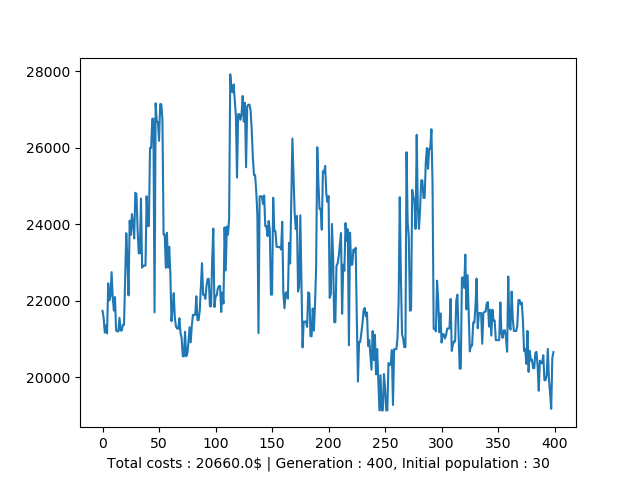
\includegraphics{image_genetic_airplane_1}
\end{center}

This graph shows you for every generation, the best cost we can get. In
the run, we run \emph{400} generations of \emph{30} individuals.

Unfortunately as you can see, the result is not converging toward a
possible solution but it is chaotic. This is because of the way we pick
our parents. We try in a first place to If we base this on the
probabilities, the results are not good.

In this first run, \(C_{T} = 0.3\) and \(M_{T}=0.15\) and
\(min_{cost}=20660\$\)

\pagebreak

In order to get around this problem, we decided to change the way of
picking the parents responsible to generate the future generation.
Instead of picking them according to there probability, we directly pick
the two best element of the population. So we change the fourth step of
the algorithm by this :

\begin{center}
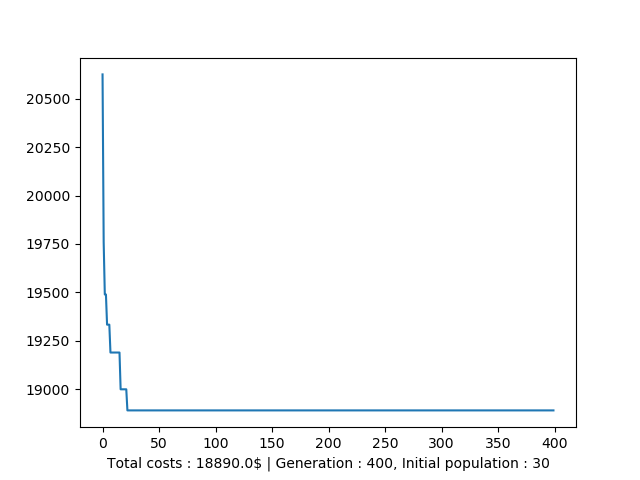
\includegraphics{image_genetic_airplane_2}
\end{center}

\textbf{4. Pick the to best members \(\{p_1,p_2\}\) of the population
according to their cost. The parents with the lowest cost among all the
population. They will be our two \emph{parents}:
\(p_1 = \underset{x \in P}{min}\ f(x) \quad \textrm{and} \quad p_2 = \underset{x \in P-{p_1}}{min}\ f(x)\).}

As you can see we have a convergence toward one of the possible solution
and no more chaos.

In this second run, \(C_{T} = 0.3\) and \(M_{T}=0.15\) and
\(min_{cost}=18980\$\)

\pagebreak

    \hypertarget{parameters-optimization}{%
\subsection{Parameters optimization}\label{parameters-optimization}}

In order to pick the appropriates arguments for the genetic stochastic
approach, I run multiple times a a range of simulation with different
parameters :

\hypertarget{statistic-representation}{%
\subsubsection{Statistic
representation}\label{statistic-representation}}

\begin{center}
(vertical = number of generation ; horizontal = population size)
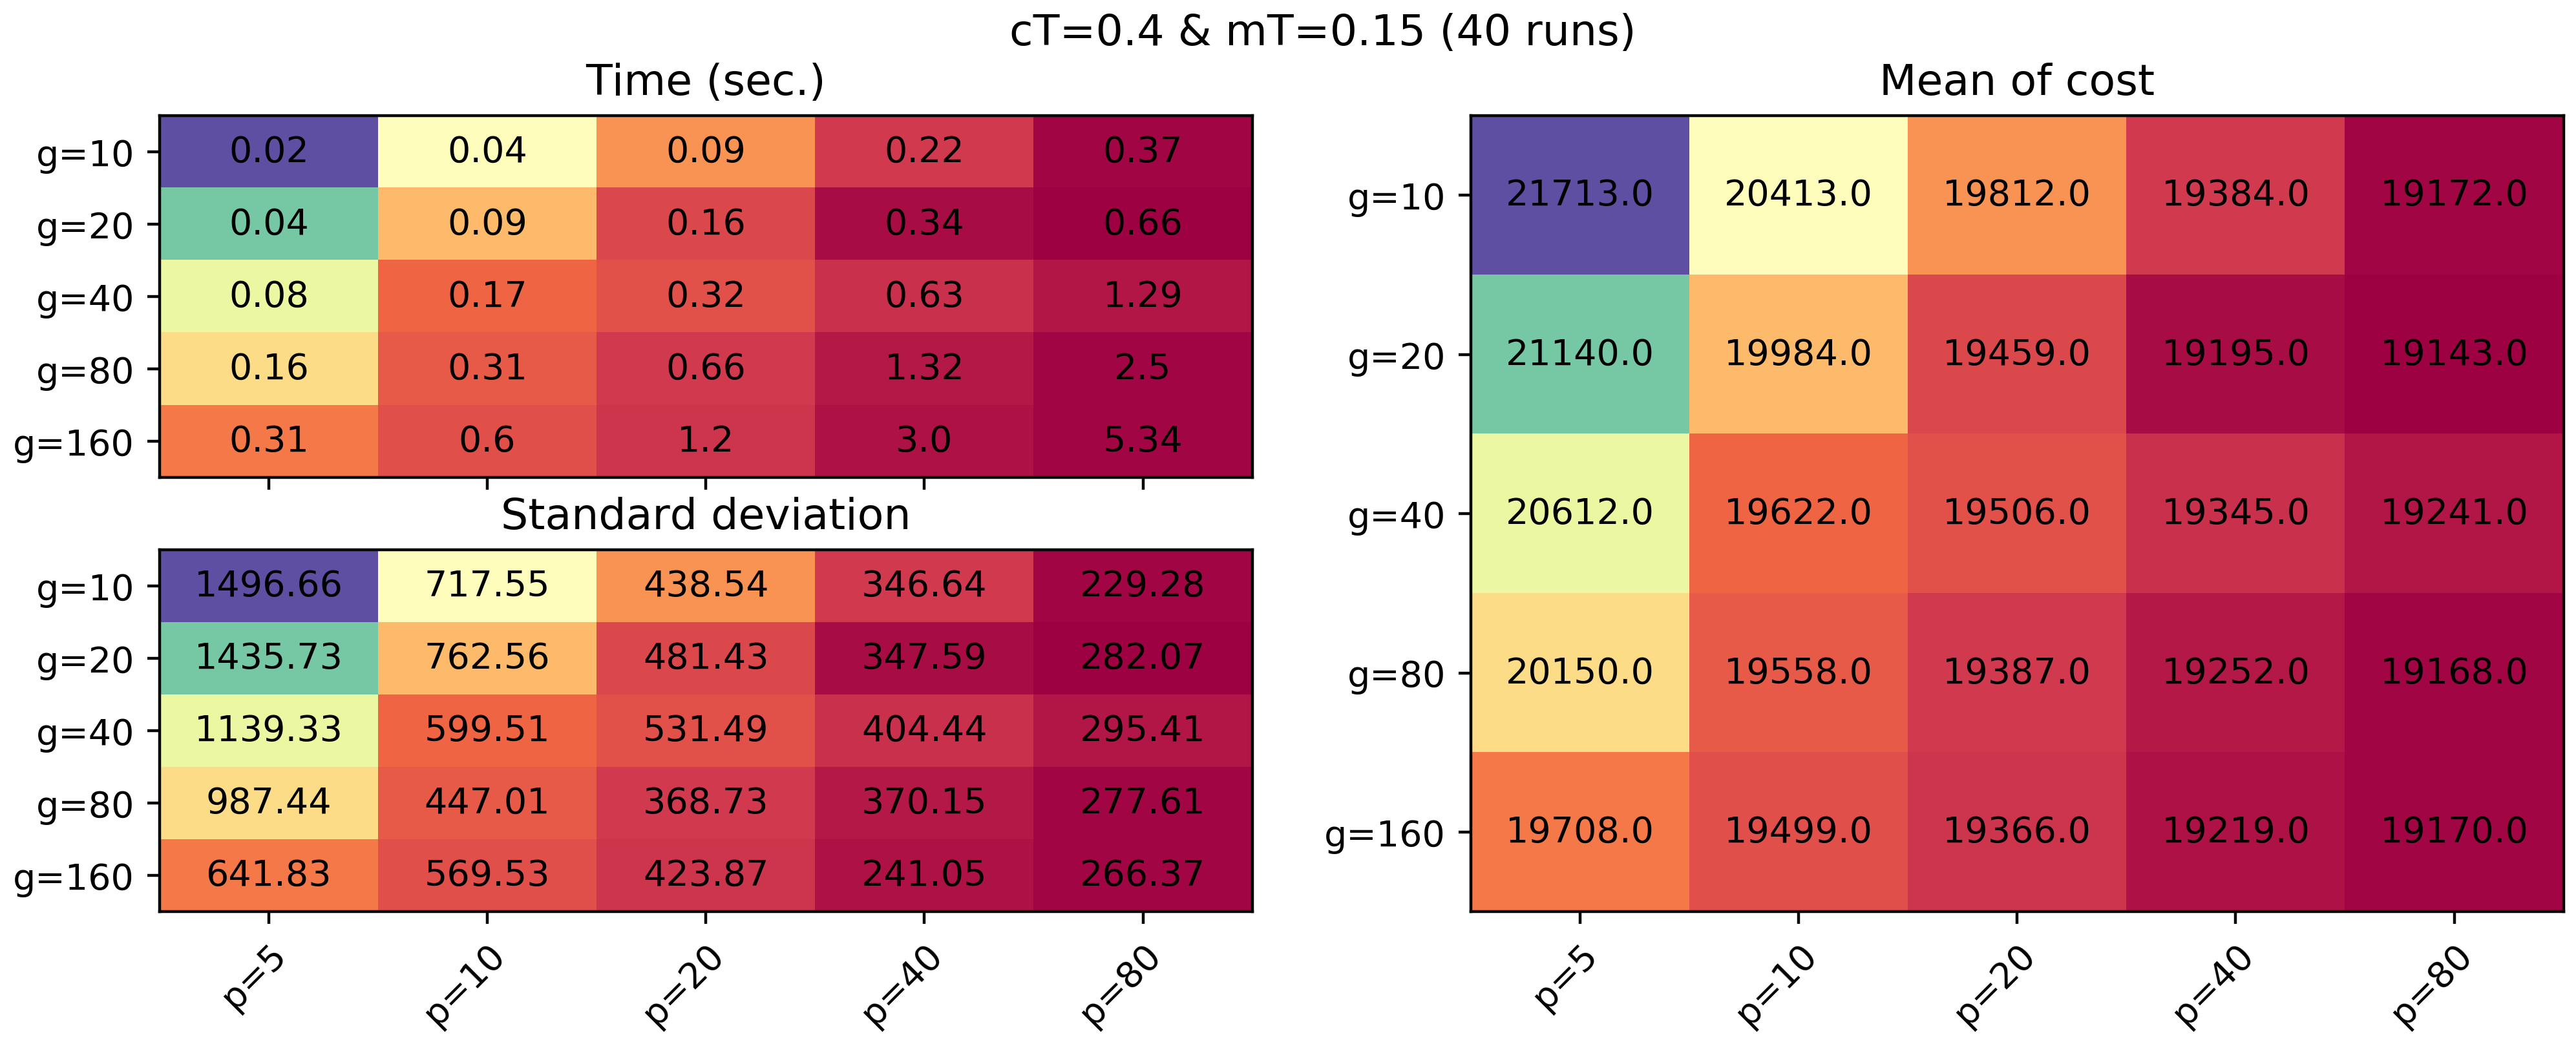
\includegraphics{image_genetic_table_1}
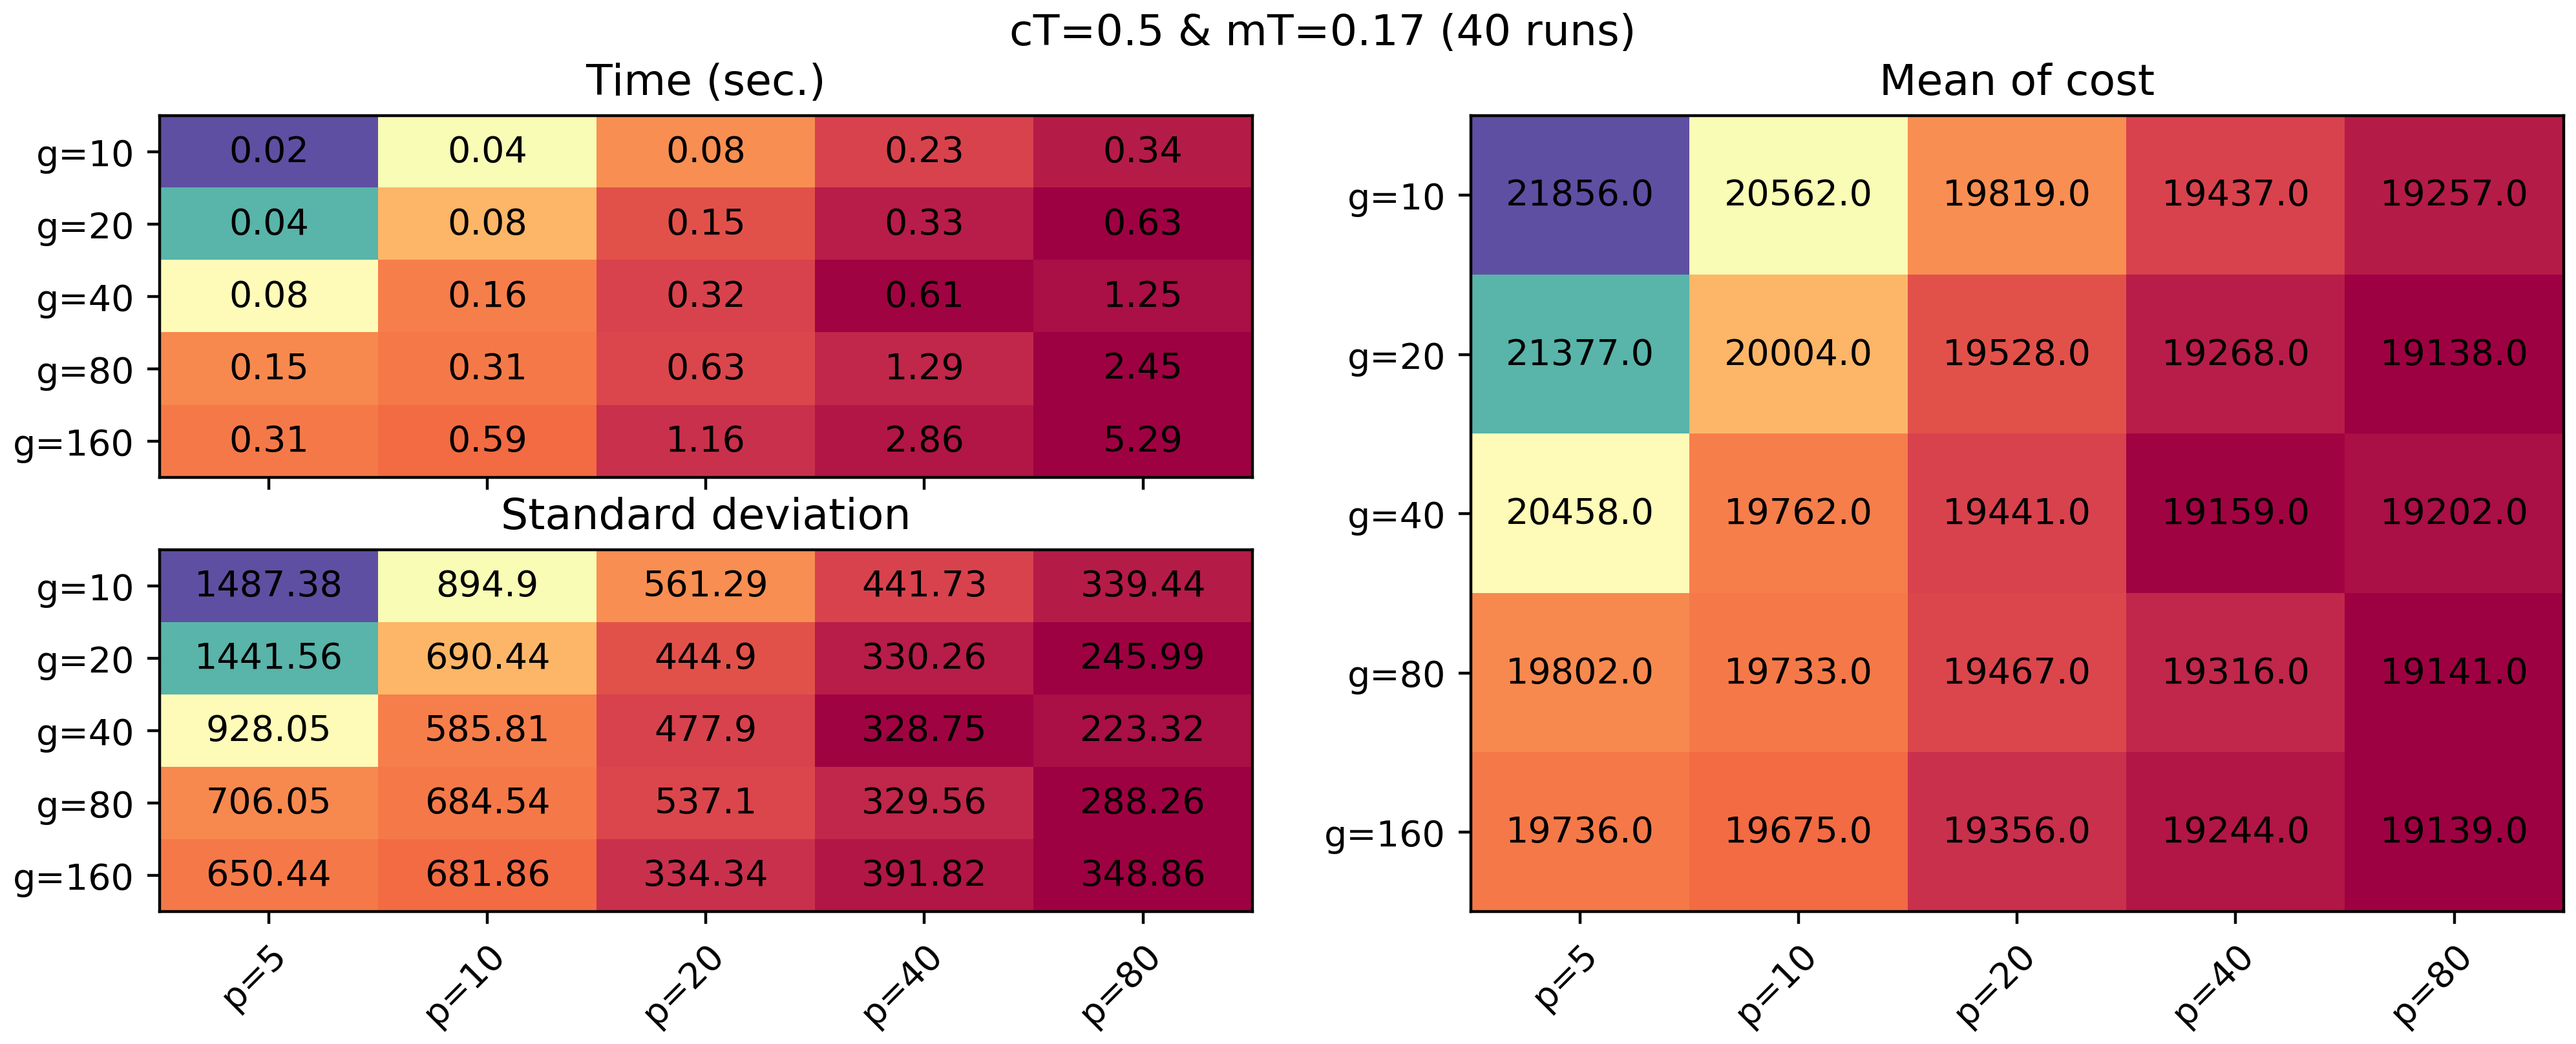
\includegraphics{image_genetic_table_2}
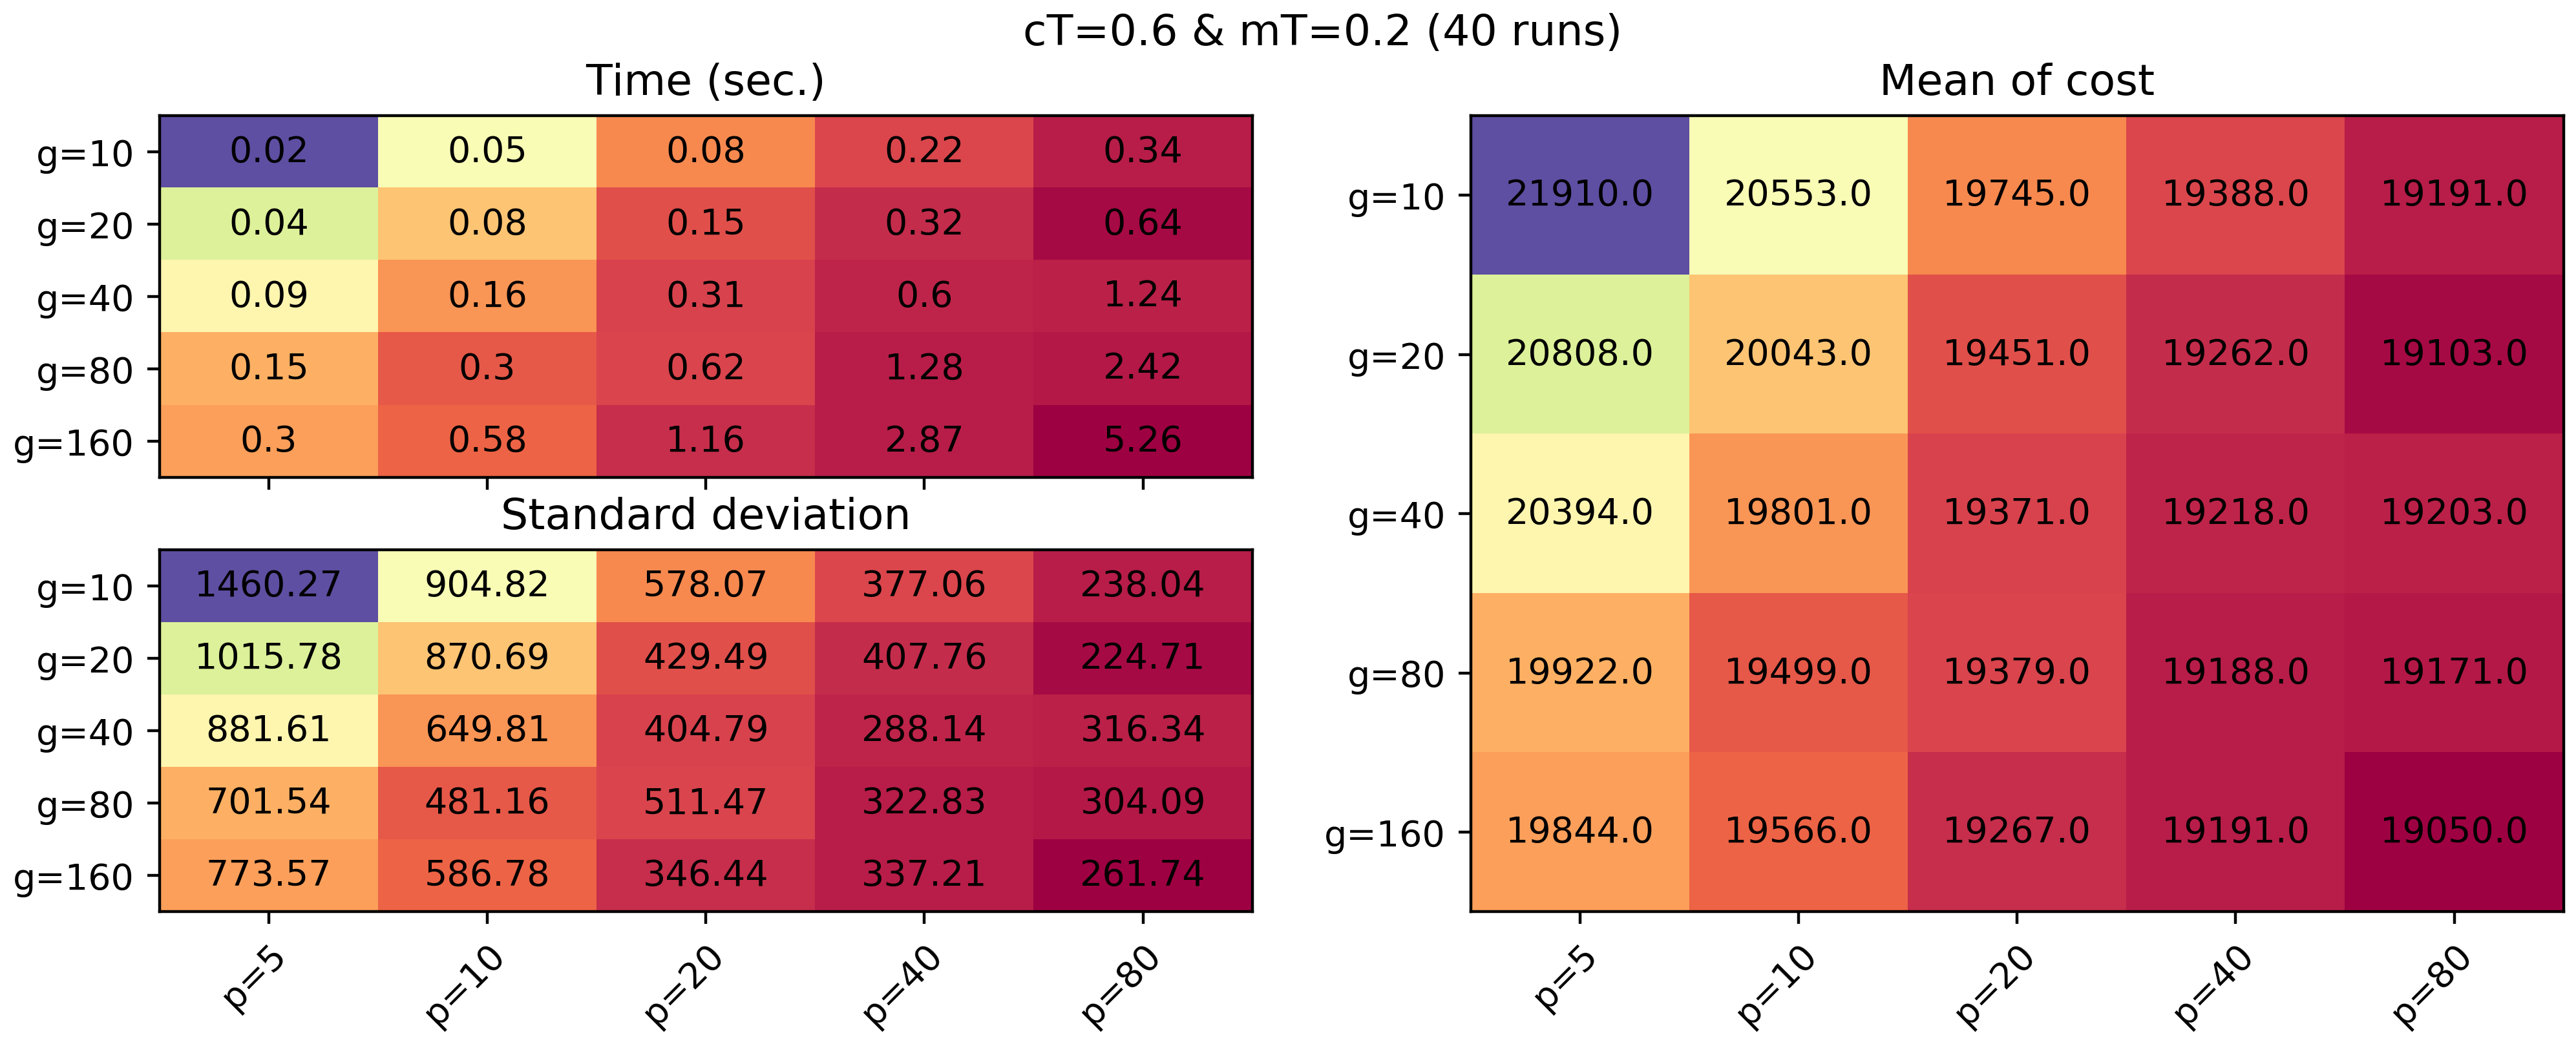
\includegraphics{image_genetic_table_3}
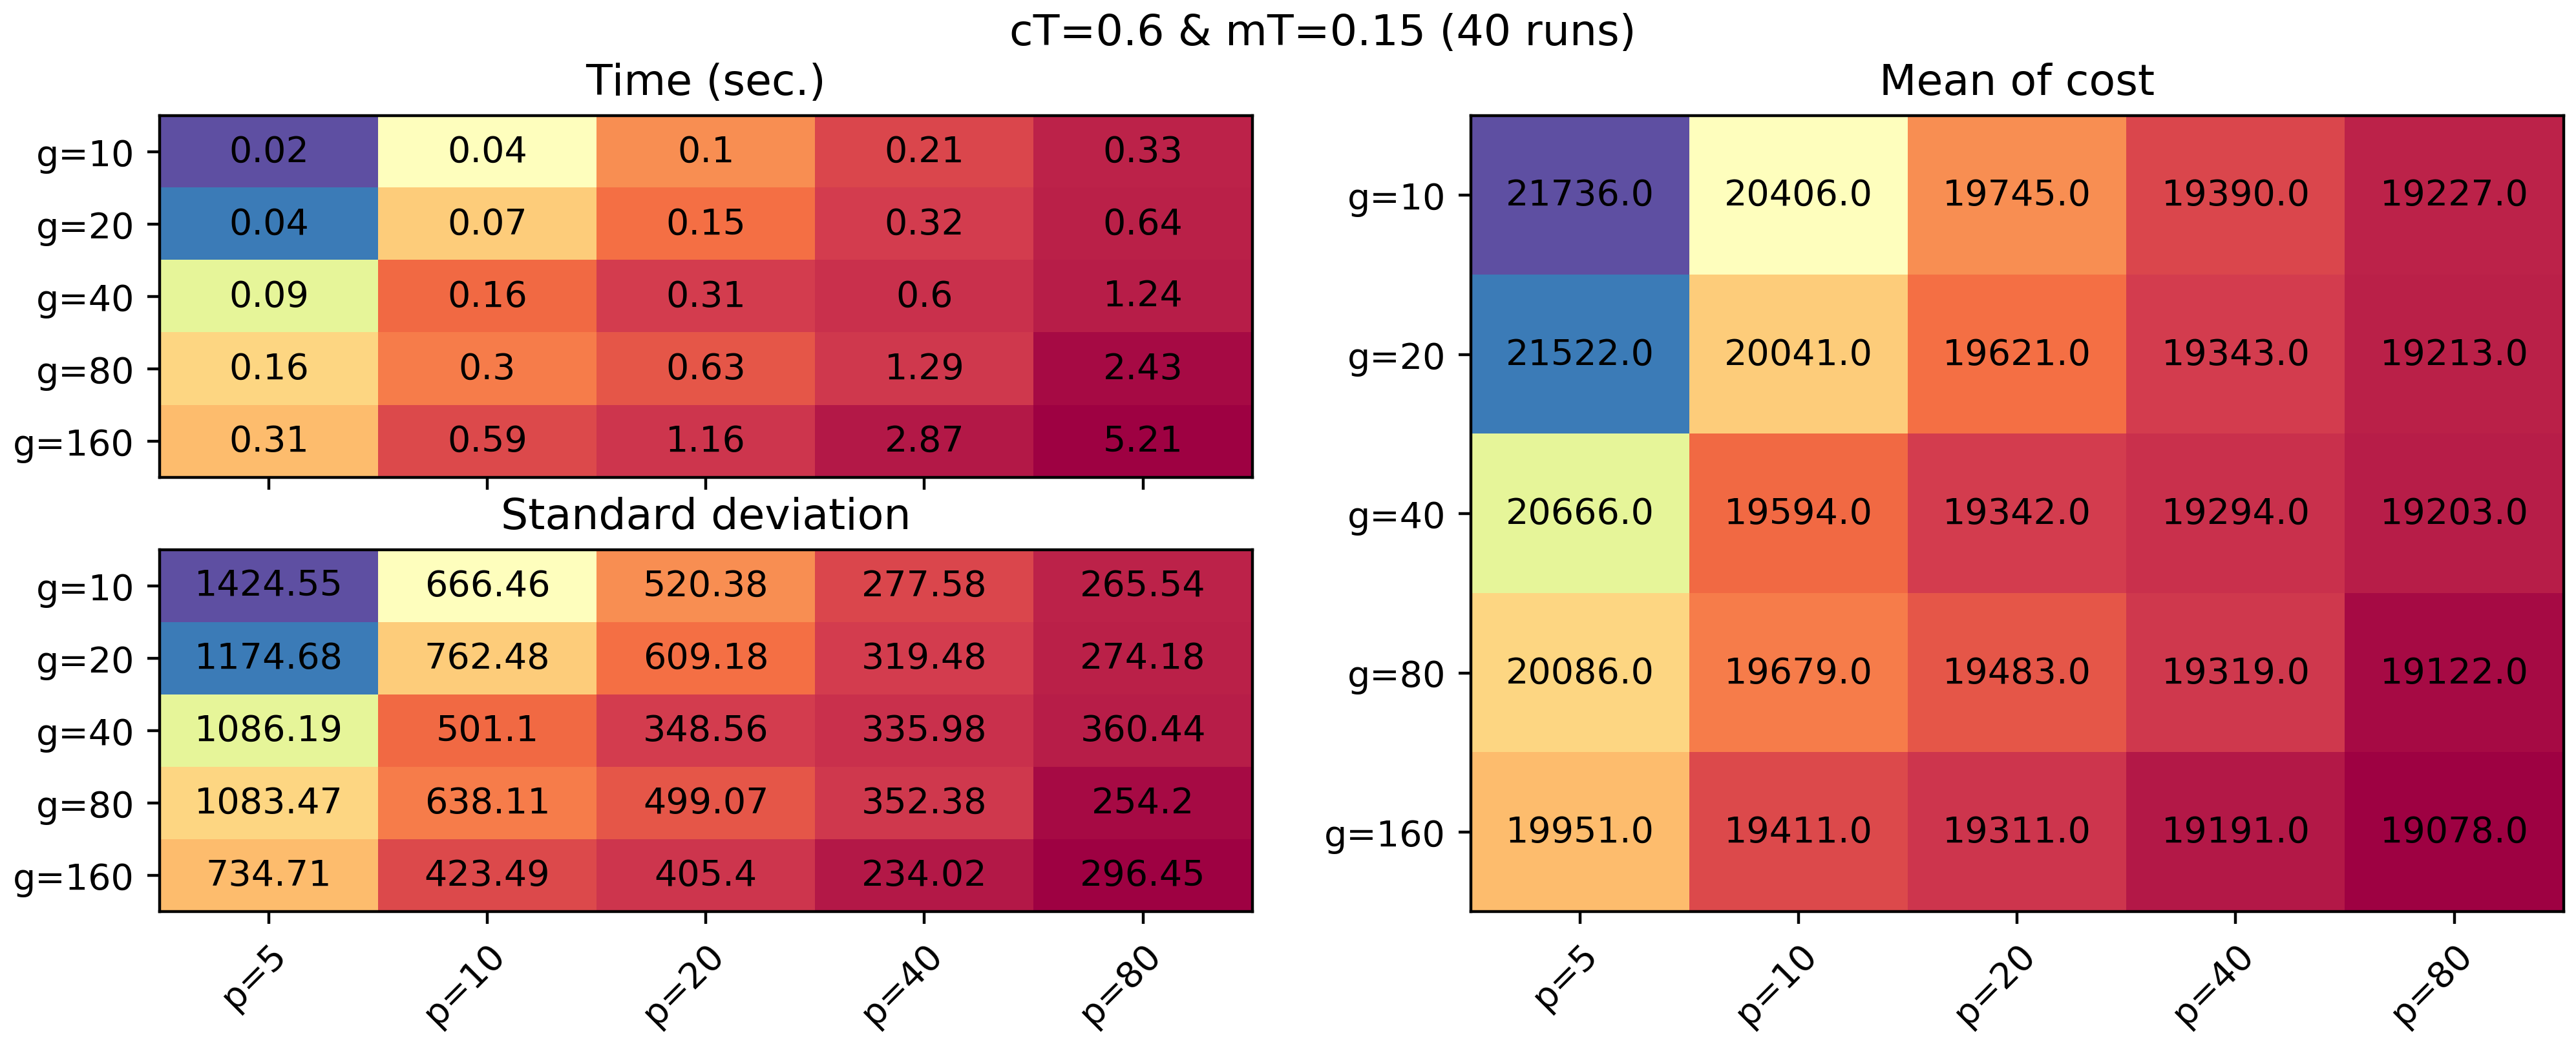
\includegraphics{image_genetic_table_4}
\end{center}

\hypertarget{decision}{%
\subsubsection{Decision}\label{decision}}

As you can see, the last runs with \(C_{T}=0.6\) and \(M_{T}=0.2\) gave
us the best result

\hypertarget{evaluation}{%
\subsubsection{Evaluation}\label{evaluation}}

When we run the algorithm with the following arguments, we get this
graph :

\begin{center}
\(n = 160\ p = 80\ C_{T}=0.6\ M_{T}=0.2\)
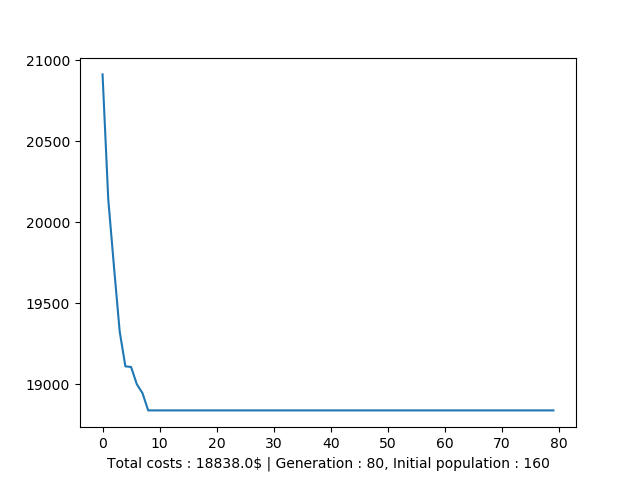
\includegraphics{image_genetic_airplane_3}
\end{center}

As we can see, there is a very quick convergence

    \hypertarget{second-proposed-solution---simulated-annealing}{%
\subsection{Second proposed solution - Simulated
Annealing}\label{second-proposed-solution---simulated-annealing}}

The simulated annealing is a good choice when one is trying to find a
single best solution to a problem, and this is the case with this
aircraft allocation problem.

\hypertarget{key-features}{%
\subsubsection{Key features}\label{key-features}}

\begin{itemize}
\tightlist
\item
  \textbf{Temperature} : The main parameters for the simulated annealing
  algorithm, the temperature allows this algorithm to have a lot of
  diversity at the beginning to finally converge to a unique solution.
\item
  \textbf{Decrease Factor} : At each end of a loop the temperature is
  multiplied by (1 - Decrease Factor), thus the decrease factor define
  the speed of convergence of this algorithm.
\item
  \textbf{Number of neighbors generated each time} : To implement a
  successful S.A. algorithm we needed to generate some neighbors from a
  given solution to create diversity and thus help the algorithm to find
  the best solution. The number of neighbors generated each time will
  remain the same : 4.
\end{itemize}

\hypertarget{the-algorithm}{%
\subsubsection{The algorithm}\label{the-algorithm}}

\hypertarget{pseudo-code}{%
\paragraph{Pseudo code}\label{pseudo-code}}

\begin{center}
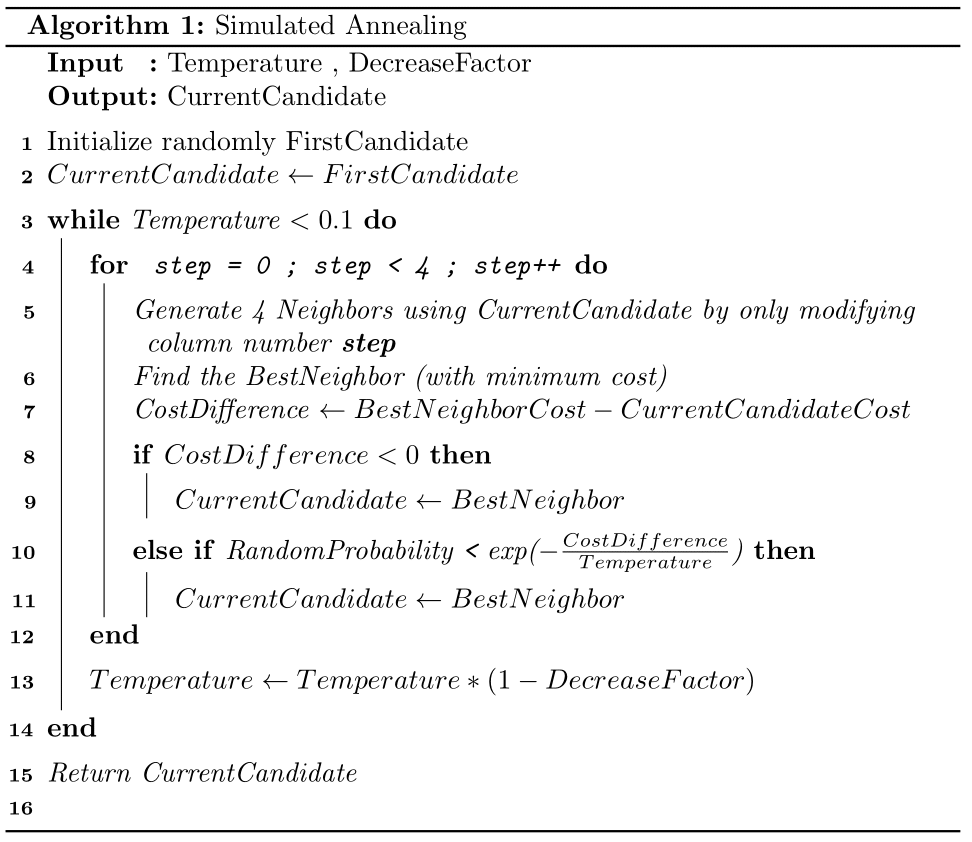
\includegraphics{sa_algo}
\end{center}

(RandomProbability is a number randomly generated between 0 and 1.)

\hypertarget{neighbors-generation}{%
\paragraph{Neighbors generation : }\label{neighbors-generation}}

Let's explain more precisely how the neighbours are generated. First, as
displayed in the pseudo code, there is not only 1 step in the S.A.
algorithm before the decreasing of the temperature but 4. We choose this
to simplify the neighbors generation and to modify airplane allocation
one airplane type at a time, so as there are 4 airplane type it is done
4 times.

There are 3 operations to generate neighbors, and they all keep the same
amount of plane as constraint :

\begin{itemize}
\tightlist
\item
  Single Random Permutation

  \begin{itemize}
  \tightlist
  \item
    Ex : From (2,\textbf{1},3,0,\textbf{4}) to
    (2,\textbf{4},3,0,\textbf{1}) ( 4 and 1 permuted)
  \end{itemize}
\item
  Random +1 / -1

  \begin{itemize}
  \tightlist
  \item
    ex : from (2,1,3,\textbf{0},\textbf{4}) to
    (2,1,3,\textbf{1},\textbf{3})
  \end{itemize}
\item
  Whole New Column

  \begin{itemize}
  \tightlist
  \item
    Ex : from (2,1,3,0,4) to (3,0,3,2,2) (whole new allocation)
  \end{itemize}
\end{itemize}

Thanks to this 3 operations the S.A. algorithm is capable of creating
enough diversity to converge towards a better and better candidate.

\pagebreak

    \hypertarget{parameters-optimization}{%
\subsection{Parameters Optimization}\label{parameters-optimization}}

The algorithm work as expected, however we also need to find the good
set of parameters for our problem in order to have the best result in
the minimum time.

\hypertarget{result}{%
\subsubsection{Result}\label{result}}

Here is some result with the cost of the current candidate in ordinate
and the number of loop in the while loop in abscissa.

\begin{center}
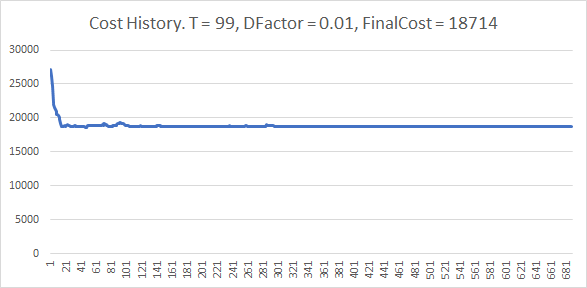
\includegraphics{sa_99_01}
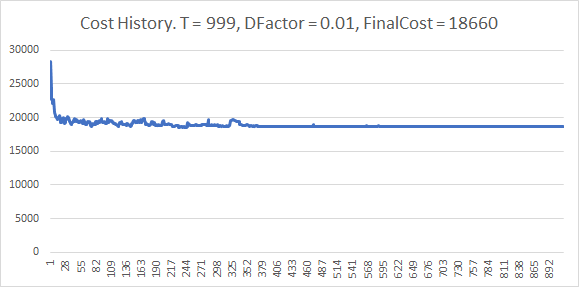
\includegraphics{sa_999_01}
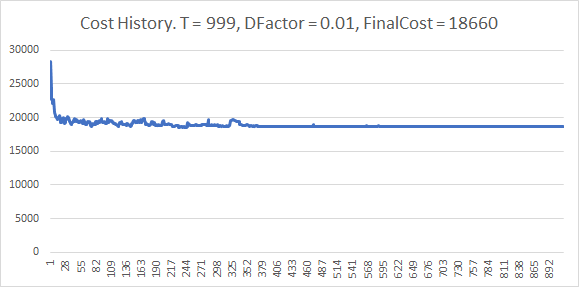
\includegraphics{sa_999_01}
\end{center}

\hypertarget{some-statistical-datas}{%
\subsubsection{Some statistical datas}\label{some-statistical-datas}}

In order to understand in a more effective way how the Temperature and
the decrease factor influences the result, we realize some statistical
computation. There is below some data using 200 output of the algorithm
per case (so the SA algorithm ran 3200 times for these data). In green
the minimum value and in red the maximum value.

\begin{center}
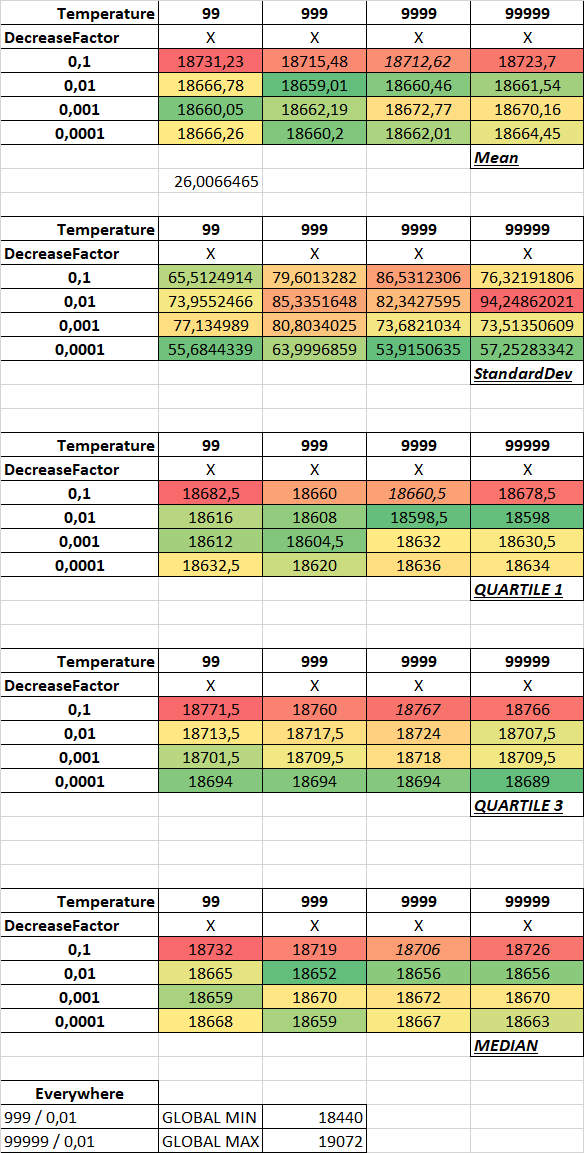
\includegraphics[width=10cm]{images/sa_datas}
\end{center}

\hypertarget{decision}{%
\subsubsection{Decision}\label{decision}}

In the statistical data we can see that (99,0.1) is obviously the worst
solutions as the algorithm has not enough time to create diversity in
order to find the best solutions and move away from local minimum.
Looking at the mean and the median the couple (999,0.01) seems to be
pretty good, but if we look at the first and third quartile it is
possible to see that (9999,0.01) and (9999,0.0001) seem to also give
good result. Finally, even if (9999,0.01) and (9999,0.0001) seem to be
good candidate, (9999,0.01) takes more than twice loop than (999,0.1)
and (9999,0.0001) more than ten times.

\textbf{\emph{So the best set of parameters for the Simulated Annealing
is Temperature = 999 and DecreaseFactor = 0.01}}.

\pagebreak

    \hypertarget{solutions-evaluation}{%
\subsection{Solutions evaluation}\label{solutions-evaluation}}

\hypertarget{intro}{%
\paragraph{Intro}\label{intro}}

In order to compare the Genetic Algorithm and the Simulated Annealing
solutions, it has been decided to compare them using the same element
which will represent the cost of each solutions : the number of times the
cost evaluation is done. In the code is will be how many times the cost
evaluations function is called.

\hypertarget{simulated-annealing}{%
\subsubsection{Simulated Annealing}\label{simulated-annealing}}

As the cost of the algorithm was defined as the number of times the cost
evaluation is done, here is the mean value and standard deviation for the
S.A. algorithm with the previous set of parameters (999,0.01). The
evaluation is done by counting the number of times the cost evaluation is
done until the algorithm find a candidate which has a cost \(<= 18 700\).
For these values the S.A. algorithm ran more than 300 times.

\textbf{\emph{S.A. cost, Mean Value : 3225\\
S.A. cost, Standard Deviation : 1582}}

This numbers may seem big, however they don't represent the number in
abscissa showed above in the Result section. In the graphics this is the
number of loop in the While Loop and in each While Loop 4 new candidate
are generated 4 times. So in each while loop the cost evaluation is
done 16 times. So if we divided these number by 16 (Mean Value : 201 /
Standard Deviation : 98 ), we have more relevant numbers to compare with
the graphic.

\hypertarget{genetic-algorithm}{%
\subsubsection{Genetic Algorithm}\label{genetic-algorithm}}

As we can see in the different runs, the best mean value we can get is
around 19100. So in order to determine the number of cost function call,
I will look how many generations does it take to get get a cost below
19200 with the following parameters :

\(n = 160\ p = 80\ C_{T}=0.6\ M_{T}=0.2\)

\begin{center}
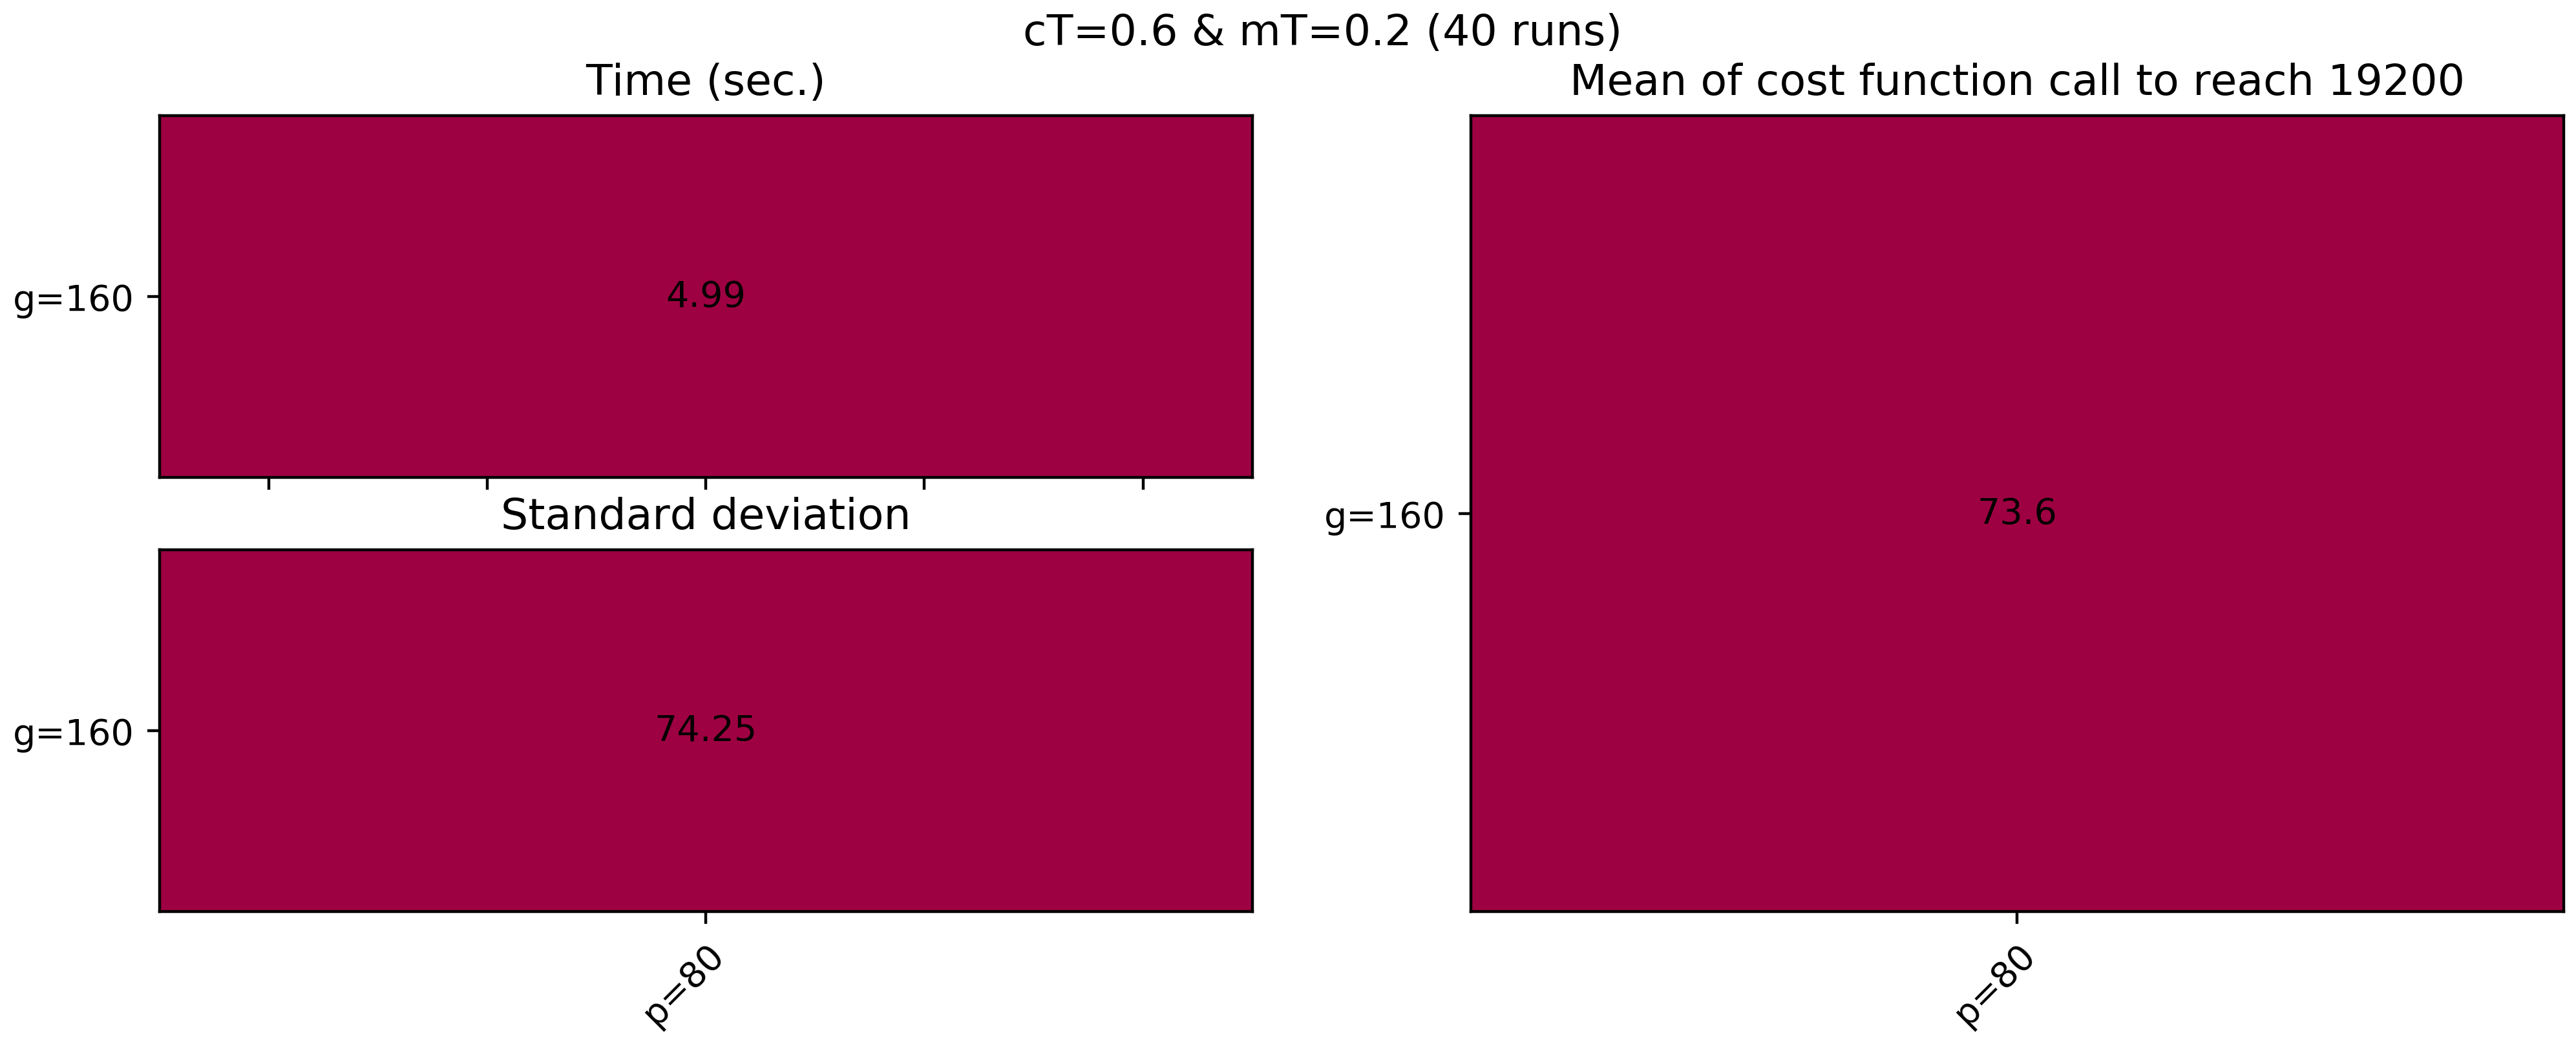
\includegraphics{images/image_genetic_table_5}
\end{center}

If we compare these values with the number of the simulated annealing
approach, we get much fewer calls. Even if we get a slightly lower cost
with the first approach \textbf{(18700 vs 19200)}, the genetic one if
much cheaper in term of computing cost.

    \hypertarget{conclusion}{%
\section{Conclusion}\label{conclusion}}

The airline sector his one of the most competitive in the world. Because of that, every cost that may be cut have to. In order to do that, many solutions to evaluate the profitability of a model exist. In our, we choose to evaluate a given model using two stochastic algorithm : Simulated Annealing and the genetic population based. From that, we decided to evaluate which of both may be the best fitted for our needs which are being able to get an aircraft distribution with the lowest cost possible. 

In order to do that, we run with both methods multiple simulation in order to pick the best parameters for each implementation. When these arguments has been chosen, we fixed then and run the final simulation and counted how much the cost function has been called during the computation. The lower this number, the more effective the algorithm is. 

We get these results : 

\begin{center}
    \(Simulated\ annealing=201\ and\ Genetic\ population\ based=74\ (mean\ of\ 40\ runs)\)
\end{center}
    
It can be seen that the genetic population based algorithm require fewer call to the cost function than the simulated annealing one. However, it's important to underline that the second methods one get slightly better results (18652) than the first one (18838)
    
To conclude, we can say that our researches brought out that **the best algorithm to pick in term of computational cost is the genetic** one. However its important to highlight that we get a slightly lower cost with the simulated annealing and also that other stochastic approach may have be better (ant colony for example)



    % Add a bibliography block to the postdoc
    
    
    
\end{document}
